The effect of including the sPHENIX support structures in the simulation, namely the sPHENIX magnet pole tip doors and IHCal support structure ring, are studied by comparing the reconstructed level \detdeta results from data to that from simulation with and without these support structures simulated. 
The reconstruction level \detdeta for the IHCal-only and OHCal-only measurements are shown in Figure \ref{fig:hcal_pole_tip_door_comparison}. 
Here a comparison between the reconstructed level \detdeta from data and EPOS simulation with and without pole tip doors simulated is shown.
The simulation with pole tip doors on better reproduces the shape of the HCal detector response seen in data, particularly in the wings of the \detdeta distribution ($|\eta| < 0.5$ in OHCal and $|\eta| < 0.8$ in IHCal).

\begin{figure}
    \centering
    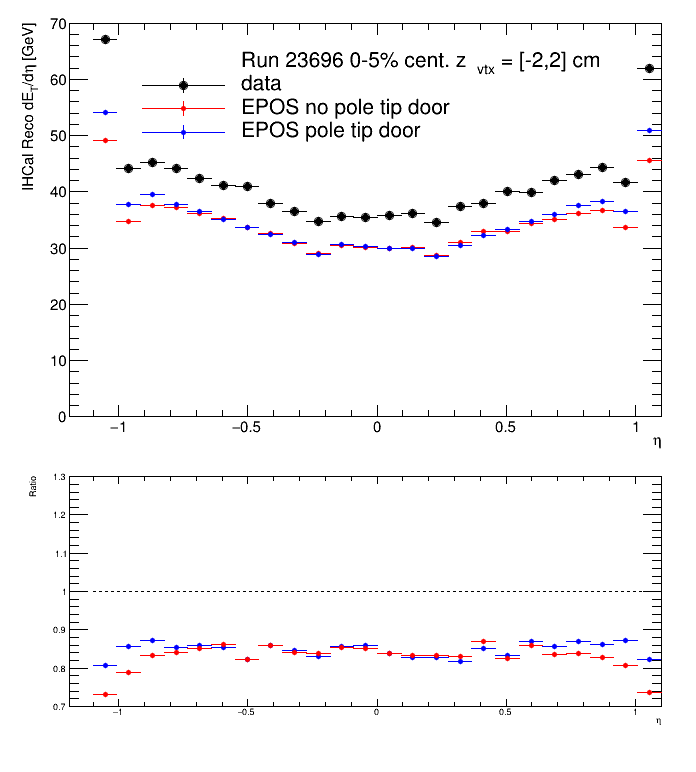
\includegraphics[width=0.48\linewidth]{detdeta/Figures/pole_tip_doors/ihcal_reco_0-5_epos_plugdoor_z=0_wratio.png}
    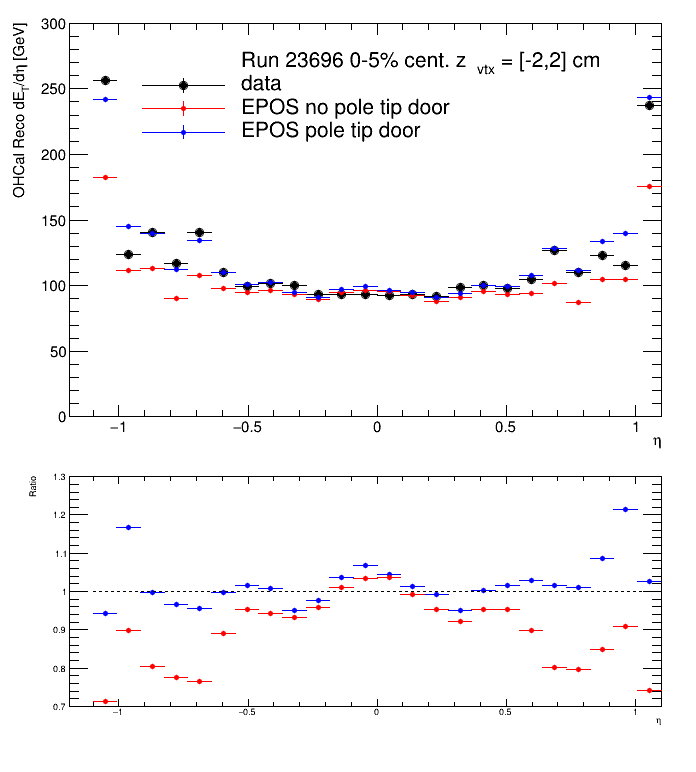
\includegraphics[width=0.48\linewidth]{detdeta/Figures/pole_tip_doors/ohcal_reco_0-5_epos_plugdoor_z=0_wratio.png}
    \caption{Plots made with ana.389p004 and privately generated EPOS simualtion (with timing bug)}
    \label{fig:hcal_pole_tip_door_comparison}
\end{figure}

In Figure \ref{fig:hcal_pole_tip_door_comparison}, there is still a remaining disagreement between the data and simulation OHCal detector response seen at $|\eta| ~ 1$ in the OHCal \detdeta distribution.
Investigation into the engineering documents of the the IHCal support structure revealed that there are support ring components mounted on the face of the towers in the OHCal at $|\eta| ~ 1$ which were not included in the simulation.
The simulation was updated to include these support ring components and the \detdeta result from simulation correction factors with and without these support ring components were compared.
Figure \ref{fig:ihcal_support_structure_comparison} shows the comparison of the fully corrected \detdeta results using correction factors which does not have the support ring geometry included (labeled "HIJING run 101") and which does have the support ring geometry included (labeled "HIJING run 14").
The discontinuity originally seen in the OHCal \detdeta measurement at $|\eta|$ = 1.0 is no longer present in the OHCal \detdeta measurement when using correction factors from the simulation with the support ring geometry included.

\begin{figure}
    \centering
    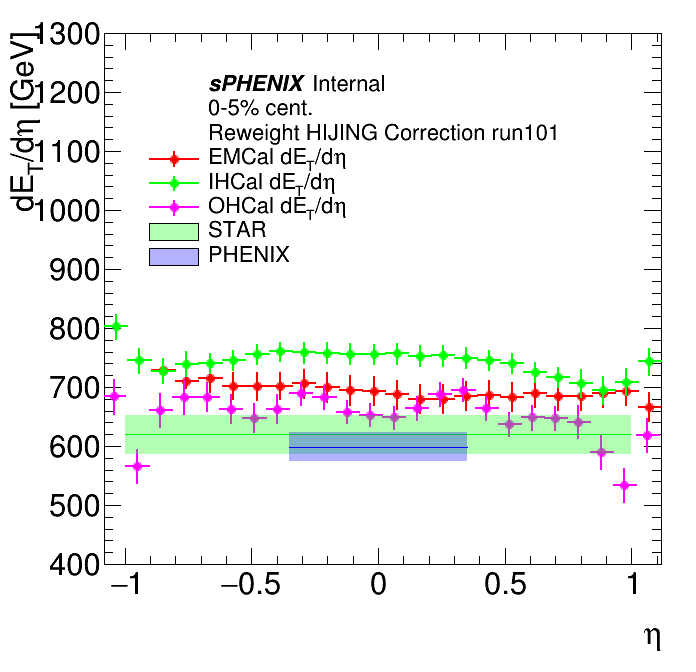
\includegraphics[width=0.48\linewidth]{detdeta/Figures/ihcal_support_structure/detdeta_reweight_hijing_run101_0-5.png}
    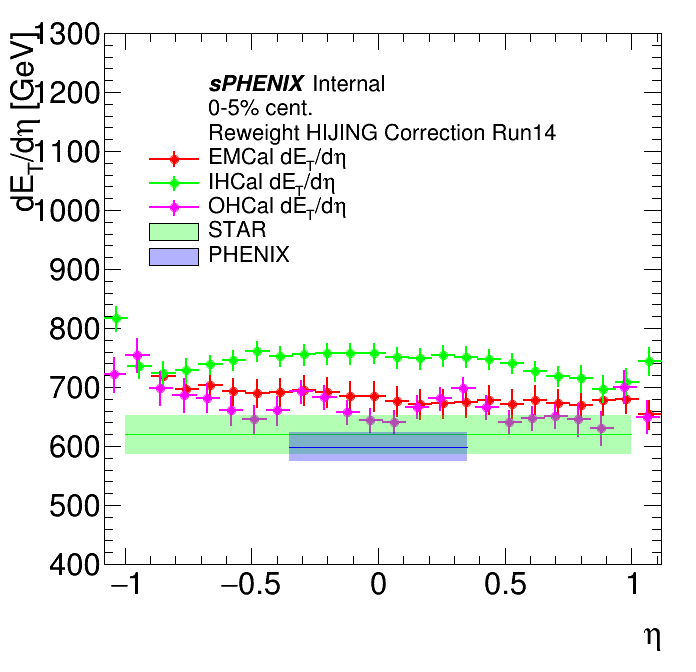
\includegraphics[width=0.48\linewidth]{detdeta/Figures/ihcal_support_structure/detdeta_reweight_hijing_run14_0-5.png}
    \caption{Comparison of fully corrected \detdeta measurements using correction factors from HIJING run 101 (left) and HIJING run 14 (right). The OHCal \detdeta measurement at $|\eta|$ = 1.0 dips in the HIJING run 101 plot due to data and MC geometry mismatch is rectified in the OHCal \detdeta measurement in the HIJING run 101 plot.}
    \label{fig:ihcal_support_structure_comparison}
\end{figure}